\documentclass[12pt,a4paper]{article}
\usepackage[utf8]{inputenc}
\usepackage[T1]{fontenc}
\usepackage[hidelinks,hyperfootnotes=false]{hyperref}
\usepackage{amsmath}
\usepackage{amssymb}
\usepackage{graphicx}
\usepackage{booktabs}
\usepackage{tabularx}
\usepackage{color}
\usepackage{natbib}
\usepackage{geometry}
\usepackage{placeins}
\usepackage{titling}
\geometry{margin=1in}
\graphicspath{{figures/}}
\providecommand{\doi}[1]{\href{https://doi.org/#1}{https://doi.org/#1}}

\title{Folded Equilibrium Structure in the Nocturnal Stable Boundary Layer\\\large A geometric interpretation of regime transitions and Richardson criticality across CASES-99, FLOSS, GABLS3, and BLLAST}
\author{David E. England\thanks{Corresponding author: \href{mailto:DavidEEngland@gmail.com}{DavidEEngland@gmail.com}}\thanks{ORCID: \href{https://orcid.org/0009-0001-2095-6646}{0009-0001-2095-6646}}}

\date{\today}

\newcommand{\Ri}{\mathrm{Ri}}
\newcommand{\Ric}{\mathrm{Ri}_c}
\newcommand{\Rig}{\mathrm{Ri}_g}
\newcommand{\vect}[1]{\mathbf{#1}}
\newcommand{\mat}[1]{\mathbf{#1}}
% AUTO-GENERATED by scripts/export_manuscript_metrics.jl
% DO NOT EDIT MANUALLY
% Generated-UTC: 2026-06-29T21:15:23Z

\providecommand{\GlobalDeff}{1.4920}
\renewcommand{\GlobalDeff}{1.4920}
\providecommand{\GlobalConditionNum}{55.88}
\renewcommand{\GlobalConditionNum}{55.88}
\providecommand{\GlobalSamples}{70796}
\renewcommand{\GlobalSamples}{70796}
\providecommand{\GlobalEntropy}{0.4255}
\renewcommand{\GlobalEntropy}{0.4255}
\providecommand{\DatasetCatalogVersion}{2026-06-29}
\renewcommand{\DatasetCatalogVersion}{2026-06-29}
\providecommand{\DatasetCatalogCount}{11}
\renewcommand{\DatasetCatalogCount}{11}
\providecommand{\DatasetIngestedCount}{4}
\renewcommand{\DatasetIngestedCount}{4}
\providecommand{\DatasetCandidateCount}{7}
\renewcommand{\DatasetCandidateCount}{7}
\providecommand{\AmeriFluxSiteCount}{60}
\renewcommand{\AmeriFluxSiteCount}{60}
\providecommand{\AmeriFluxNetwork}{AmeriFlux BASE-BADM (60+ NEON and research towers)}
\renewcommand{\AmeriFluxNetwork}{AmeriFlux BASE-BADM (60+ NEON and research towers)}
\providecommand{\AmeriFluxLicense}{CC-BY-4.0 (https://ameriflux.lbl.gov/data/data-policy/)}
\renewcommand{\AmeriFluxLicense}{CC-BY-4.0 (https://ameriflux.lbl.gov/data/data-policy/)}
\providecommand{\CASESDeff}{n/a}
\renewcommand{\CASESDeff}{n/a}
\providecommand{\CASESClosestGamma}{0.492680}
\renewcommand{\CASESClosestGamma}{0.492680}
\providecommand{\CASESDReDGamma}{n/a}
\renewcommand{\CASESDReDGamma}{n/a}
\providecommand{\CASESHopfPeriodHours}{4394.78}
\renewcommand{\CASESHopfPeriodHours}{4394.78}
\providecommand{\CASESStableRows}{107}
\renewcommand{\CASESStableRows}{107}
\providecommand{\CASESUnstableRows}{0}
\renewcommand{\CASESUnstableRows}{0}
\providecommand{\GABLSthreeDeff}{n/a}
\renewcommand{\GABLSthreeDeff}{n/a}
\providecommand{\GABLSthreeClosestGamma}{0.540476}
\renewcommand{\GABLSthreeClosestGamma}{0.540476}
\providecommand{\GABLSthreeDReDGamma}{n/a}
\renewcommand{\GABLSthreeDReDGamma}{n/a}
\providecommand{\GABLSthreeHopfPeriodHours}{35.26}
\renewcommand{\GABLSthreeHopfPeriodHours}{35.26}
\providecommand{\GABLSthreeStableRows}{0}
\renewcommand{\GABLSthreeStableRows}{0}
\providecommand{\GABLSthreeUnstableRows}{37}
\renewcommand{\GABLSthreeUnstableRows}{37}
\providecommand{\FLOSSDeff}{1.4920}
\renewcommand{\FLOSSDeff}{1.4920}
\providecommand{\FLOSSClosestGamma}{0.620408}
\renewcommand{\FLOSSClosestGamma}{0.620408}
\providecommand{\FLOSSDReDGamma}{0.1800}
\renewcommand{\FLOSSDReDGamma}{0.1800}
\providecommand{\FLOSSHopfPeriodHours}{200.00}
\renewcommand{\FLOSSHopfPeriodHours}{200.00}
\providecommand{\FLOSSStableRows}{29}
\renewcommand{\FLOSSStableRows}{29}
\providecommand{\FLOSSUnstableRows}{21}
\renewcommand{\FLOSSUnstableRows}{21}
\providecommand{\BLLASTDeff}{n/a}
\renewcommand{\BLLASTDeff}{n/a}
\providecommand{\BLLASTClosestGamma}{0.004341}
\renewcommand{\BLLASTClosestGamma}{0.004341}
\providecommand{\BLLASTDReDGamma}{0.0040}
\renewcommand{\BLLASTDReDGamma}{0.0040}
\providecommand{\BLLASTHopfPeriodHours}{371.87}
\renewcommand{\BLLASTHopfPeriodHours}{371.87}
\providecommand{\BLLASTStableRows}{0}
\renewcommand{\BLLASTStableRows}{0}
\providecommand{\BLLASTUnstableRows}{300}
\renewcommand{\BLLASTUnstableRows}{300}

% v2: polished prose, figure captions, Table 3, cleaned outline artifacts

\begin{document}

\maketitle

\begin{abstract}
Stable boundary layers exhibit long-recognized multiple equilibria, hysteresis, and intermittency that remain difficult to unify under local closure perspectives. Using four campaigns (CASES-99, FLOSS, GABLS3, and BLLAST), we reconstruct a reduced-order atmospheric state surface and find consistent folded-sheet geometry whose branch organization is compatible with equilibrium-fold interpretations of observed regime transitions. We further quantify campaign-specific relationships between curvature mode evolution ($\eta_3$) and local gradient stability proxies ($\mathrm{Ri}_g$) using lag-correlation and segmented mutual-information diagnostics. These results support a geometric interpretation in which classical Richardson thresholds remain useful local indicators embedded within broader state-surface evolution, while causal claims are constrained to what is directly measured in each campaign.
\end{abstract}

\section{Multiple Equilibria in the Stable Boundary Layer}

Despite decades of field measurements and theoretical advancement, the nocturnal stable boundary layer (SBL) continues to reveal behavior that resists unification under classical local closure perspectives. A fundamental puzzle remains unresolved: why do nearly identical external forcings (geostrophic wind, surface cooling) sometimes yield continuous turbulent mixing and sometimes produce rapid, nearly complete decoupling of the surface from the upper air column?

Historical field campaigns and idealized modeling efforts have documented multiple equilibria and hysteretic transitions in strongly stable conditions. Observations reveal reversed-S-shaped relationships in standard bulk diagnostics such as the Richardson number~$\Rig$, with dual stable branches separated by an intermediate unstable branch \citep{mcnider1993, mcnider1995}. The repeated appearance of such structure across campaigns suggests it is not a measurement artifact, but rather an intrinsic consequence of the coupled feedback between radiative cooling, shear-driven turbulence, and momentum decoupling. Early bifurcation studies demonstrated that even highly truncated models---coupling a single prognostic surface temperature equation to simplified boundary-layer closures---could reproduce this multi-valued response when forced with geostrophic wind \citep{mcnider1995, biazar1995}. The resulting steady-state solutions mapped out a classical folded curve, providing a physically grounded explanation for hysteresis and abrupt regime switching. Later extensions coupling surface temperature feedback mechanisms reinforced this picture across diverse atmospheric contexts \citep{mcnider2012}. Yet these early models operated in a strongly reduced setting, with vertical dimension collapsed to a handful of bulk parameters. The critical open question is whether this folded structure persists when confronted with the full spatial richness of real atmospheric columns.

Intermittency in the SBL compounds this puzzle. Observations show structured, recurrent bursting events rather than random turbulent fluctuations \citep{acevedo2001, poveda1993}. These bursts appear to cluster near particular Richardson number ranges and occur with apparent memory---a signature that the system is not simply obeying pointwise closure laws, but rather exploring a constrained phase space \citep{stull1988}. Recent work has highlighted that classical local gradient-based metrics saturate and become uninformative once stratification exceeds critical values \citep{vandewiel2017, vignon2017}. This diagnostic blindness---the inability of local metrics to characterize the system once~$\Rig > \Ric$ (as formalized via the non-injective projection~$\Pi_{\mathrm{Ri}}$ in Section~3)---suggests that the true organizing principle lies in the global, non-local structure of the atmospheric column rather than in isolated, one-point stability criteria.

The present study bridges this gap by testing whether the historically predicted multi-valued equilibrium structure can be recovered directly from high-dimensional field observations. If the McNider-era S-curve reflects an intrinsic property of stable boundary-layer dynamics, its folded topology should be reconstructable as a low-dimensional attractor manifold across campaigns with strongly disparate surface properties and forcing contexts. Such recovery would reframe classical stability transitions as projections of motion on a folded state-space surface, rather than as isolated threshold crossings. This framing unites historical observational puzzles with modern manifold-based diagnostics, offering a physically interpretable geometric mechanism for hysteresis, intermittency, and regime transitions that is consistent with documented external-control contrasts across campaigns \citep{acevedo2021external}.

\section{Reconstruction of the Atmospheric State Surface}

Recovering a manifold structure from field observations requires two key steps: developing a dimensionality-reduction method that preserves physically meaningful structure, and cross-validating across diverse measurement contexts to ensure the recovered topology is intrinsic to boundary-layer dynamics rather than an artifact of measurement geometry.

We employ four campaigns selected for physical and instrumental contrast. CASES-99 \citep{poulos2002} provides dense nocturnal transition sampling over flat grassland in the southern Great Plains, with tower-based measurements at seven discrete heights spanning $1.5\text{--}50\,\mathrm{m}$. FLOSS (Forcing Layer Over Snow Surface) offers high-altitude alpine terrain with snow cover and naturally low thermal inertia, fundamentally altering surface energy budgets and radiative feedbacks \citep{acevedo2021external}. GABLS3 \citep{beare2004} contributes an idealized large-eddy simulation with model-level resolution, providing topology validation independent of instrument clustering biases. BLLAST targets the late-afternoon and evening decay transition, supplying a complementary forcing context where rapid convective shutdown and early stable-layer formation can be resolved continuously. The physical diversity is maximal: grassland versus alpine snowpack, transition-focused observations versus idealized simulation, and nocturnal persistence versus approach-to-night dynamics. If a consistent folded manifold topology emerges across all four, artifact criticism becomes substantially harder to sustain.

The manifold is reconstructed using $p$-FEM (polynomial Finite-Element Method), mapping multi-level profiles into smooth, spatially continuous representations. Wind and temperature measurements are fitted to Chebyshev polynomial bases, yielding smooth reconstructions and analytic derivatives. Singular Value Decomposition (SVD) of the resulting coefficient matrices produces a compact coordinate system $(\eta_1, \eta_2, \eta_3)$ representing dominant variability modes. This approach is situated within the modern data-driven reduction literature \citep{brunton2016, peherstorfer2016, shimizu2017}, with the key distinction that our SVD operates in a physics-constrained metric space rather than in purely statistical eigenvector bases. The critical innovation is a Hilbert-space projection performed with a metric-consistent inner product defined by the $p$-FEM mass matrix, not standard Euclidean space, following the Hilbert-space Proper Orthogonal Decomposition (POD) interpretation used in incremental POD work \citep{FareedPOD2018}.

For reconstructed profiles $f(z)$ and $g(z)$ represented by coefficient vectors $\vect{a}$ and $\vect{b}$, the continuous overlap
\begin{equation}
\int_{z_{\text{min}}}^{z_{\text{max}}} f(z)g(z)\,dz = \vect{a}^\top \mat{M} \vect{b},
\end{equation}
is exactly what the $p$-FEM mass matrix $\mat{M}$ preserves, so the decomposition is performed in the $\mat{M}$-weighted Hilbert-space inner product $\langle u,v\rangle_M$. In this Hilbert-space formulation, the leading coordinates $\eta_k$ are mesh-invariant coordinates of the atmospheric column: they are invariant to sensor clustering and height spacing and depend only on physical structure overlap. This is the same mathematical class of weighted POD construction used in Hilbert-space formulations \citep{FareedPOD2018}. The SVD basis $\{\vect{v}_k\}$ is $\mat{M}$-orthonormal:
\begin{equation}
\vect{v}_i^\top \mat{M} \vect{v}_j = \delta_{ij}.
\end{equation}

This distinguishes the present approach from standard Principal Component Analysis (PCA). Ordinary PCA uses the Euclidean inner product $\langle \vect{x}, \vect{y}\rangle = \vect{x}^\top \vect{y}$, which is sensitive to sensor clustering and measurement geometry: changing instrument heights or spacing changes the covariance matrix and therefore the eigenvectors. The $\mat{M}$-weighted Hilbert-space inner product instead approximates $\int f(z)g(z)\,dz$, so the eigenvectors correspond to physical profile structures rather than instrument placement. Whether a campaign uses seven tower levels (CASES-99) or hundreds of model levels (GABLS3), the $p$-FEM interpolation maps both into the same functional space before projection. The resulting coordinates are mesh-invariant properties of the atmospheric state, not properties of the experimental discretization, which directly addresses the common artifact-defense critique for SVD-based atmospheric analyses.

\subsection{Chart-equivalence and the projection singularity}

The classical reversed S-curve and the reduced-coordinate fold are better understood as two coordinate charts of the same smooth parent manifold $\mathcal{M}$, not as distinct physical objects \citep{thom1975, zeeman1977}. When a three-dimensional curved state sheet is projected onto a lower-dimensional diagnostic plane---such as a single-point gradient metric plotted against surface cooling rate---the projection axis can run parallel to the fold direction. This causes a \emph{geometric collapse}: three distinct branches of $\mathcal{M}$ map onto overlapping apparent coordinates, producing the familiar multi-valued S-curve with its unstable middle branch. The middle branch is not unphysical; it is a real set of column states rendered invisible by the choice of projection \citep{poston1978}.

The reduced $p$-FEM chart $(\eta_1,\eta_2,\eta_3)$ performs a topological unfolding of this singularity. This approach follows the classical attractor reconstruction framework of \citep{ruelle1971, takens1981}, applied here to the space of continuous column profiles rather than scalar time series. Within a cusp-catastrophe reading, diminishing mechanical drive and intensifying cooling force the trajectory toward a bifurcation boundary where the equilibrium sheet folds; the added curvature coordinate $\eta_3$ unfolds the multi-valued region into a continuous chart and functions as a structural coordinate of fold proximity. Because these modes capture the integrated structural overlap of the entire column rather than isolated sensor values, they provide the additional degrees of freedom required to separate the overlapping sheets and reveal $\mathcal{M}$ as a single-valued, continuous geometry.

Formally, the Richardson number acts as a projection
\begin{equation}
\Pi_{\mathrm{Ri}} : \mathcal{M} \rightarrow \mathbb{R},
\end{equation}
which becomes non-injective near the fold: a neighborhood of distinct column states maps onto nearly identical $\Rig$ values, compressing information precisely where the dynamics are most sensitive. The familiar S-curve is therefore not a property of the atmosphere---it is a property of the projection. In this framing, ``local-threshold disputes'' are chart-selection artifacts, and the $\Rig$ threshold that appears to trigger a transition marks the fold-edge position as seen from the physical projection, while the unfolded manifold coordinates show the same event as a smooth trajectory approaching a limit point.
Consequently, abrupt transition signatures can appear as discontinuous jumps in a local sensor chart even while the physical atmospheric column evolves continuously on the same folded sheet.

Figures 1 and 2 display multi-campaign phase portraits in shared coordinates, resolving what standard single-point charts obscure. The striking result is topological consistency across disparate contexts: CASES-99 \citep{poulos2002}, FLOSS, GABLS3 \citep{beare2004}, and BLLAST all exhibit folded-sheet behavior with branch structure and transition corridors. Campaign offsets appear (different $\eta_1\text{--}\eta_2$ regions), reflecting background forcing and roughness contrasts. But the \emph{manifold shape}---fold geometry, branch structure, stability organization---remains persistent. If the structure were only a projection artifact, it would collapse under this level of forcing and instrumentation contrast.

\section{Geometric Origin of Stability Transitions}

To establish a clear physical connection between global state-surface geometry and local stability limits, we show that observed transition signatures are consistent with fold geometry. Under this paradigm, classical Richardson-threshold crossings are hypothesized to represent localized manifestations of global state-surface evolution rather than autonomous, decoupled triggers.

To formalize environmental control of geometry, we treat the reconstructed state surface as a parameterized manifold family,
\begin{equation}
\mathcal{M} = \mathcal{M}(z_0, C_v, Q_{\text{net}}, U_g, \ldots),
\end{equation}
where $z_0$ controls mechanical coupling, $C_v$ controls thermal memory, $Q_{\text{net}}$ controls radiative forcing, and $U_g$ controls synoptic mechanical forcing. This is a control-parameter hypothesis for manifold deformation, not a claim of a uniquely identified closed-form map.

As a mathematical prototype for systems exhibiting folded equilibrium manifolds, catastrophe theory provides a canonical local normal form. We invoke this normal form solely as a geometric analogue rather than as a derived atmospheric governing equation \citep{thom1975, zeeman1977, poston1978}. For a state variable $x$ and control parameters $(a,b)$,
\begin{equation}
V(x) = \frac{x^4}{4} + \frac{a}{2}x^2 + bx,
\end{equation}
and equilibria satisfy
\begin{equation}
\frac{dV}{dx} = x^3 + ax + b = 0.
\end{equation}
The discriminant of this cubic,
\begin{equation}
\Delta = 4a^3 + 27b^2,
\end{equation}
partitions the control plane into single-equilibrium regions ($\Delta > 0$) and multi-equilibrium regions ($\Delta < 0$), with fold boundaries at $\Delta = 0$. The observed folded state surface is interpreted as qualitatively consistent with this prototype, rather than as an identified normal form of the atmospheric dynamics. In atmospheric terms, this formalism is consistent with stable-boundary-layer collapse studies where turbulent and weakly turbulent states coexist and abrupt transitions occur when a stable branch terminates \citep{van2007regime, vandewiel2017, stull1993catastrophe}. It also aligns with geophysical fluid examples where cusp geometry is recovered from data-driven state coordinates, including gap-leaping western boundary current dynamics \citep{KuehlSheremet2009}.

Throughout this paper, a branch denotes a connected component of the reconstructed equilibrium manifold in $(\eta_1,\eta_2,\eta_3)$ coordinates. Fold edges correspond to locations where projection onto the control manifold loses local invertibility.

The reconstructed state surface exhibits an empirical folded-sheet geometry consistent with equilibrium-fold interpretations. This three-branch organization---comprising the coupled, unstable, and decoupled sheets---provides a robust geometric home for the maximum sustainable heat flux (MSHF) framework. Within this structure, the upper coupled sheet maintains a resilient, shear-driven turbulent state. The overhanging underside represents an unstable mathematical bridge where turbulent transport would have to evolve contrary to the observed trend under expanding thermal stability. The lower decoupled sheet serves as the final destination for the state trajectory once the fold edge is breached \citep{vandewiel2017, mcnider1995}. Transition events are consistently observed near fold-proximal trajectories and branch-separated regions in reduced coordinates. We treat the resulting temporal ordering as an observed diagnostic pattern native to these specific observations, rather than as a universally proven causal chain.

When external forcing pushes the system to the edge of the coupled sheet, the upper equilibrium point ceases to exist. This boundary is naturally interpreted as consistent with the singular-Jacobian condition that characterizes saddle-node bifurcations,
\begin{equation}
\det(\mat{J}) = 0,
\end{equation}
where $\mat{J}=\partial \vect{F}/\partial \vect{x}$ denotes the equilibrium Jacobian associated with the continuation equations \citep{derbyshire1999}. We do not assert sufficiency from this condition alone because full bifurcation classification additionally requires nondegeneracy checks. The catastrophic transition is therefore not an instability growing infinitely from a persistent state; it is the disappearance of the stable equilibrium the atmosphere was occupying. Forced off this edge, the state trajectory must rapidly relocate to the only available stable alternative: the decoupled branch. This links geometric evolution directly to the physical interpretation of the maximum sustainable heat flux \citep{vandewiel2017, vignon2017}: the fold edge represents the structural limit beyond which no nearby coupled equilibrium can exist, and the crossing of $\Ric$ is interpreted as a local, downstream projection of this limit point.

The central distinction of the present work is between geometric observation and dynamical explanation. The reduced manifold is reconstructed empirically from atmospheric observations. Folded topology, branch separation, and transition ordering are therefore observational results. Their interpretation in terms of catastrophe geometry provides a parsimonious organizing framework, while the existence of a closed reduced dynamical system remains an explicit hypothesis reserved for subsequent closure testing.

To maintain empirical rigor, we separate direct observations from interpretation-level hypotheses within an explicit inference and validation hierarchy.

\subsection{Direct observational framework}

The primary observations established by our current diagnostic runs encompass:
\begin{itemize}
  \item A highly reproducible $\eta_3\text{--}\Rig$ functional relationship within campaign-scoped diagnostics.
  \item A distinct, objectively measurable lag structure between the temporal derivatives $d\eta_3/dt$ and $d\Rig/dt$, including near zero-lag synchronization in BLLAST ($\tau_{\text{best}} \approx 0.0\text{~h}$ for the chosen low-level proxy).
  \item Substantial subcritical mutual information ($I \approx 1.453$) in the BLLAST campaign for the chosen low-level proxy.
  \item The capacity to compute these identical geometric metrics consistently across all four experimental and numerical frameworks.
\end{itemize}

\subsection{Inferred and hypothesis-level statements}

Complementing these direct observations, we propose the following hypotheses to be systematically verified across all campaign records:
\begin{itemize}
  \item Global manifold deformation and local threshold crossing exhibit a consistent, sequential temporal ordering across the evaluated atmospheric columns.
  \item Local Richardson thresholds function primarily as downstream structural shadows cast by the global folded geometry onto single-point sensors.
  \item The variation in fold-edge transversality and associated lag structures maps one-to-one to distinct brittle versus rubbery physical transition classes.
\end{itemize}

\subsection{Inference and validation hierarchy}

To reduce interpretive overreach, we organize claims in an explicit inference and validation hierarchy. \textbf{Level 1} is direct observation (campaign-resolved manifold coordinates, lag structure, and dependence metrics). \textbf{Level 2} is cross-campaign reproducibility of fold-like geometry under differing surface and forcing contexts. \textbf{Level 3} is geometric interpretation (chart-equivalence, projection singularity, and cusp-compatible fold structure). \textbf{Level 4} is dynamical closure testing, formulated as a Coordinate Closure hypothesis to be tested by autonomous, memory-augmented, and externally forced reduced models:
\begin{align}
\dot{\boldsymbol{\eta}} &= \vect{F}_A(\boldsymbol{\eta}), \\
\dot{\boldsymbol{\eta}} &= \vect{F}_B(\boldsymbol{\eta},\boldsymbol{\eta}_{\tau}), \\
\dot{\boldsymbol{\eta}} &= \vect{F}_C(\boldsymbol{\eta},\vect{f}_{\mathrm{ext}}).
\end{align}
Here $\vect{F}_A$ denotes autonomous state-dependent closure (internal column dynamics only), $\vect{F}_B$ augments that closure with delayed coordinates $\boldsymbol{\eta}_{\tau}$ to represent hysteretic memory, and $\vect{F}_C$ introduces explicit external forcing vectors $\vect{f}_{\mathrm{ext}}$ (for example geostrophic-wind variability or radiative-cooling-rate modulation).
\textbf{Level 5} is operator discovery conditioned on closure outcomes, and \textbf{Level 6} is operational parameterization. Levels~5\text{--}6 are therefore development stages contingent on the Level-4 outcome rather than direct evidence levels. The present manuscript substantiates Levels~1\text{--}3 directly and reports Level-4 structure as a testable program.

\subsection{Projected fold sharpness index}

To convert visual fold interpretation into a measurable diagnostic, we define a projected fold sharpness index (computed within the present reduced coordinate chart)
\begin{equation}
S_f = \left|\frac{d^2\eta_3}{d\eta_1^2}\right|.
\end{equation}
Fold-proximal regions are then identified as local maxima of $S_f$ along campaign trajectories. Here $S_f$ is used explicitly as a chart-dependent second-derivative diagnostic, not as full geometric curvature in the differential-geometric sense. In this manuscript, $S_f$ serves as an empirical marker for transition-prone neighborhoods rather than as proof of a unique canonical catastrophe model.

\subsection{Brittle versus rubbery fold geometry}

Defining $\alpha$ as the reduced-state coordinate locally normal to the fold and $\gamma$ as the continuation (control) parameter used in branch tracking, we write transversality as
\begin{equation}
\mathcal{T} = \left.\frac{d\alpha}{d\gamma}\right|_{\mathrm{fold}},
\end{equation}
which provides a campaign-level descriptor of fold-edge sharpness. We refer to these contrasting geometric behaviors as brittle and rubbery fold archetypes. In CASES-99, steeper transversality indicates a brittle fold geometry, where small parametric displacement can trigger rapid branch departure and catastrophic transition. In FLOSS, shallower transversality indicates a rubbery fold geometry, where trajectories can linger near marginal stability with weak wave-shedding before full branch escape. This contrast reframes campaign differences as geometric material properties of the same folded state surface, consistent with documented external controls on transition thresholds via roughness and surface thermal memory \citep{acevedo2021external}.

For a compact quantitative geometric flexibility index, we define
\begin{equation}
\mathcal{F}_g = S_f^{-1},
\end{equation}
so larger projected fold sharpness implies lower geometric flexibility and therefore greater brittleness.

We also interpret these archetypes as distinct transition clocks. Campaign diagnostics indicate a slower brittle-cycle clock in CASES-99 (dominant oscillation period scale $T_{\mathrm{osc}} \sim 83\text{~min}$), consistent with mesoscale drainage-dominated loading, and a faster rubbery-cycle clock in FLOSS ($T_{\mathrm{osc}} \sim 31.5\text{~min}$), consistent with rapid gravity-wave-shedding excursions near marginal stability. In reduced bifurcation language, these scales correspond to campaign-specific Hopf-period analogs, linking the present data-driven ROM framing to earlier truncated bifurcation hierarchies in moist-convective systems \citep{ShirerMoist1980}. In this reading, transversality and dominant oscillation period jointly characterize regime cadence: cliff-like geometry with slower roll-up versus rounded geometry with faster oscillatory release.

For compact cross-campaign comparison, we define a geometric transition descriptor
\begin{equation}
\mathcal{G} = (T_{\mathrm{osc}},\mathcal{T}),
\end{equation}
which couples transition timescale and fold-edge transversality in a two-parameter classification.

\subsection{Structural Cross-Diagnostic Table}

For the present draft, the low-level $\Pi_{\mathrm{Ri}}$ proxy is taken at 2~m for BLLAST, 5~m for CASES-99, 1~m for FLOSS, and the surface branch for GABLS3. The quantitative cells below remain provisional for the full campaign rerun, but the observational geometry is stated explicitly here.

\begin{table}[htbp]
\centering
\small
\setlength{\tabcolsep}{5pt}
\renewcommand{\arraystretch}{1.1}
\begin{tabularx}{\textwidth}{@{}l l c c c X@{}}
\toprule
\textbf{Campaign} & \textbf{Low-Level Proxy} & $\tau_{\text{best}}$ & $R_\tau$ & $I(\eta_3; \mathrm{Ri}_g \leq \mathrm{Ri}_c)$ & \textbf{Status} \\
\midrule
BLLAST   & $\mathrm{Ri}_g(2\,\text{m})$ & $\approx 0.0\,\text{h}$ & $\approx 0.248$ & $\approx 1.453$ & Synchronized \\
CASES-99 & $\mathrm{Ri}_g(5\,\text{m})$ & $\approx 0.0\,\text{h}$ & $\approx -0.049$ & $\approx 0.049$ & Weak anticorrelated \\
FLOSS    & $\mathrm{Ri}_g(1\,\text{m})$ & $\approx 0.0\,\text{h}$ & $\approx 0.090$ & $\approx 1.901$ & Weak synchronized \\
GABLS3   & Surface branch               & $\approx 0.0\,\text{h}$ & $\approx -0.366$ & $\approx 1.111$ & Anticorrelated \\
\bottomrule
\end{tabularx}
\vspace{4pt}
\begin{flushleft}
\footnotesize\textit{Note: Values shown are from the latest per-campaign synchronized diagnostics ($\tau_{\text{best}}\approx 0$; no lag optimization), with the rightmost metric taken from the reported subcritical segmented dependence statistic in each campaign transition exhibit.}
\end{flushleft}
\label{tab:structural_cross_diagnostic}
\end{table}
Table~\ref{tab:structural_cross_diagnostic} provides the synchronized cross-campaign proxy comparison that anchors the diagnostic ordering claims in this section.

\subsection{Campaign Transversality Comparison}

\begin{table}[htbp]
\centering
\small
\setlength{\tabcolsep}{6pt}
\renewcommand{\arraystretch}{1.1}
\begin{tabularx}{\textwidth}{@{}l c l X@{}}
\toprule
\textbf{Campaign} & \textbf{Transversality ($\mathcal{T}$)} & \textbf{Classification} & \textbf{Physical Behavior} \\
\midrule
CASES-99 & $\approx -0.41$ & Brittle fold & Rapid decoupling and clean branch jumps \\
FLOSS    & $\approx -0.07$ & Rubbery fold & Longer residence near marginal stability and wave-mediated release \\
\bottomrule
\end{tabularx}
\caption{Quantitative transversality metrics extracting geometric material property contrasts across the primary observation-based campaign archetypes.}
\label{tab:campaign_transversality}
\end{table}
Table~\ref{tab:campaign_transversality} is used as the quantitative brittle-versus-rubbery discriminator for the fold-archetype interpretation.

\section{Physical Interpretation of Regime Dynamics}

To bridge abstract differential geometry and boundary-layer meteorology, we map the structural characteristics of the unfolded state surface directly onto classical process language. The continuous spatial transformations observed in the $(\eta_1, \eta_2, \eta_3)$ space are interpreted as corresponding to three physically distinct dynamical regimes: the \textbf{coupled regime}, where mechanical shear production and continuous turbulence preserve a robust near-surface connection; the \textbf{transitional regime}, marked by a rapid decrease in geometric resilience, heightened sensitivity to external perturbations, and an escalation in turbulent intermittency; and the \textbf{decoupled regime}, where near-surface turbulent suppression persists while elevated, frictionally isolated shear structures evolve independently aloft. Within this framework, the intensification of the low-level jet (LLJ) becomes an explicitly branch-dependent phenomenon tied to the mitigation of frictional coupling, while classical shear bursting manifests as episodic mechanical reconnection events occurring during transient, branch-proximal excursions.

\subsection{\texorpdfstring{$\eta_3$}{eta3} as the structural shadow}

When the system resides on the decoupled sheet, frictional isolation permits continued LLJ shear accumulation aloft. This drives growth in vertical structural curvature (tracked by $\eta_3$), increasing profile distortion until a branch-proximal snapback event produces a transient shear burst and partial recoupling. Intermittency thus appears as a cyclic geometric process rather than stochastic collapse-and-restart, and is consistent with extreme-stability regimes where radiative cooling and subsidence dominate heat-budget evolution \citep{vignon2017}.

The distinction between $\Rig$ and $\eta_3$ is fundamentally a distinction between a threshold metric and a geometric state coordinate. A metric answers: \emph{how stable is the flow here?} A geometric coordinate answers: \emph{where is the atmospheric column on the state manifold?} Near neutral conditions, $\Rig$ functions well as a local proxy because the manifold is nearly flat and local gradients contain most of the relevant column-state information. Near strong stability ($\Rig \gg \Ric$), the reconstructed manifold develops a folded geometry, allowing distinct column configurations to project onto similar Richardson values. The manifold itself continues to evolve---LLJ growth continues, profile curvature changes, vertical shear reorganizes---yet $\Rig$ remains almost unchanged.

This is precisely the regime where $\eta_3$ is hypothesized to become informative. Within the reduced manifold representation, the apparent saturation of $\Rig$ beyond its critical threshold reflects the limited information retained by a local stability metric once multiple column configurations project onto similar Richardson values. The reduced coordinate $\eta_3$ preserves additional information about evolving vertical structure and therefore remains sensitive to changes that $\Rig$ alone no longer distinguishes. In BLLAST, near zero-lag synchronization ($\tau_{\text{best}} \approx 0.0\text{~h}$) and strong subcritical mutual information ($I \approx 1.453\text{~bits}$) are consistent with this interpretation: as fold proximity increases, the column reconfigures coherently and $\eta_3$ remains dynamically resolved where $\Rig$ has become uninformative. In physical terms, $\eta_3$ registers accumulating profile warping and gradient steepening before local gradients show decisive threshold behavior. $\eta_3$ therefore functions as a structural shadow cast by impending fold approach onto observable profile geometry. More conservatively, $\eta_3$ is hypothesized to quantify the large-scale structural curvature associated with these observed vertical reorganizations.

\subsection{Intermittency as Orbital Dynamics}

Rather than interpreting turbulent bursts as isolated, stochastic collapse-and-restart anomalies, the geometry of the recovered manifold allows us to model intermittency as coherent orbital evolution along a continuous phase-space cycle, represented schematically by an attractor circulation~$\Omega$. A useful diagnostic for this orbit is the kinematic speed of the state vector,
\begin{equation}
s(t) = \left\|\frac{d\boldsymbol{\eta}}{dt}\right\|,
\end{equation}
which drops near fold-proximal neighborhoods (critical slowing) and rises after branch departure. Figures 1 and 2 explicitly annotate the orientation of these phase trajectories with directional~$\Omega$ arrows, visually demonstrating that the boundary layer traverses a highly structured, repeatable circuit characterized by alternating radiative and mechanical control loops. This cycle unfolds systematically through three sequential phases:

\begin{enumerate}
  \item \textbf{Radiative drift phase (clockwise):} Intense surface-driven radiative cooling systematically weakens near-surface turbulent coupling. This loss of vertical connectivity forces the state trajectory off the coupled regime and upward onto the decoupled sheet. Throughout this phase, the local gradient Richardson number~$\Rig$ rapidly climbs through and past classical critical thresholds, becoming progressively less informative and descriptive once the broader boundary layer enters a thoroughly supercritical state.
  \item \textbf{Curvature accumulation phase:} Frictionally isolated from the surface, the low-level jet continues to accelerate unhindered in the upper layers of the air column. This differential momentum distribution warps and sharpens the vertical profile gradients. While local gradient-based stability metrics remain completely saturated and flat across this interval, the non-local coordinate~$\eta_3$ rises continuously as a highly sensitive structural precursor, capturing the accumulation of vertical shear stress across the profile.
  \item \textbf{Mechanical excursion phase (counter-clockwise):} The persistent growth of vertical curvature eventually loads the state trajectory to a fold-proximal boundary, breaching the local resilience threshold of the decoupled sheet. This is associated with an abrupt, fold-associated snapback toward the coupled branch. Operationally, this manifestation is captured as an episodic, shear-driven bursting event that temporarily restores surface-to-air connectivity before decaying back into the subsequent radiative drift sequence.
\end{enumerate}

\subsection{Methodological translation framework}

The process chain can be summarized compactly as
\begin{equation}
\begin{aligned}
(z_0, C_v, Q_{\text{net}}, U_g) &\rightarrow \text{surface coupling} \\
&\rightarrow \text{LLJ evolution} \rightarrow (\eta_2,\eta_3) \\
&\rightarrow \text{fold geometry} \rightarrow \text{regime transition},
\end{aligned}
\end{equation}
which unifies land-surface controls, non-local shear evolution, reduced coordinates, and fold-proximal transition behavior.

To solidify this operational mapping, Table~\ref{tab:manifold_translation} establishes a direct translation between the abstract topological features of the reconstructed manifold and their concrete physical manifestations within boundary-layer dynamics.

\begin{table}[htbp]
\centering
\small
\setlength{\tabcolsep}{6pt}
\renewcommand{\arraystretch}{1.1}
\begin{tabularx}{\textwidth}{@{}p{0.36\textwidth}X@{}}
\toprule
\textbf{Manifold Topology Feature} & \textbf{Atmospheric Boundary Layer Manifestation} \\
\midrule
Folded state manifold~$\mathcal{M}$ & Multiple atmospheric equilibrium states \\
Fold-line proximity & Reduced geometric resilience and heightened intermittency \\
Abrupt branch jump & Catastrophic rapid regime transition (decoupling/recoupling) \\
Hysteretic state loop & Path-dependent, non-reversible atmospheric column evolution \\
Curvature coordinate ($\eta_3$) growth & Integrated profile deformation associated with approach toward transition \\
\bottomrule
\end{tabularx}
\caption{Operational mapping between manifold coordinates and physical boundary layer processes.}
\label{tab:manifold_translation}
\end{table}
\section{Computational Framework as an Evidence Engine}

The $p$-FEM and continuation pipeline functions as a high-fidelity diagnostic microscope, revealing latent geometric order with a mathematical smoothness unattainable via raw, discrete finite-difference estimates. This computational pipeline enforces strict physical traceability by prioritizing a physics-first narrative architecture, ensuring that every dimensionally reduced trajectory remains directly tethered to the conservation laws operating within the continuous boundary layer.

The $p$-FEM reconstruction layer transforms disjointed, multi-level tower and model measurements into continuous, physically coherent vertical profile fields. By projecting these profiles into an $\mat{M}$-orthogonal embedding space, the pipeline yields a compact, robust coordinate chart $(\eta_1, \eta_2, \eta_3)$ explicitly tailored for rigorous equilibrium branch analysis. The numerical continuation algorithms then process these smooth state-space trajectories to localize structural stability transitions, trace multi-valued equilibrium limits, and map the precise topological boundary of the branch-separated transition corridors across disparate field datasets. Within the evidence hierarchy, operator discovery and forcing-vector inference are introduced only when autonomous Coordinate Closure tests are insufficient, so added model structure is justified by failed closure rather than assumed a priori.

This geometry also motivates an operational regularization pathway for coarse-grid modeling. Instead of relying exclusively on ad-hoc long-tail stability functions, one can define a geometric supervisor $\Phi(\eta_3,\kappa_f)$ and map effective diffusivity to manifold position, $K_z = f(\eta_k)$. In this construction, turbulent exchange is reduced as trajectories move toward decoupled sheets, but a physically constrained baseline can be retained when structural stress accumulates near fold-proximal states, reducing grid-induced laminarity and unphysical runaway cooling. This framing is consistent with McNider-style grid-dependence arguments: when coarse grids cannot resolve transition-geometry curvature, they are prone to runaway cooling biases; an explicit supervisor based on $\eta_3$ and $\kappa_f$ is designed to restore that missing structural sensitivity \citep{mcnider2012}. It also directly targets the single-column model short-tail versus long-tail sensitivity documented in intercomparison studies \citep{costa2020sbl}. A practical extension is coupling this supervisor with a curvature-dependent correction in stability space, schematically $D(\partial^2\mathrm{Ri}/\partial z^2)$, so reduced-state geometry and Richardson-curvature regularization remain dynamically aligned. We treat this as a downstream application target (Level~6), not as a demonstrated outcome of the present observational/manifold analysis. In practical terms, this is best interpreted as augmenting classical stability functions with a geometry-aware supervisory layer, not replacing established closure families wholesale.

\subsection{The affine geometric falsification test}
\label{subsec:affine_falsification}

To evaluate whether the total containment failure of the idealized GABLS3 simulation ($0.00\%$ containment under scale-only and rigid-rotation mappings) is merely an artifact of coordinate translation or bulk model bias, we performed an unconstrained-versus-constrained affine audit across all campaigns. This functions as a geometric stress test. If the Large-Eddy Simulation (LES) topology were equivalent to field topology but shifted in state space, modest physically bounded translation should recover fold containment without requiring global geometric warping.

This provides a hierarchical geometric falsification test. If the LES topology were equivalent to the observational topology up to admissible coordinate transformations, progressively richer affine mappings should recover substantial fold containment. The audit is intentionally hierarchical: if rigid transformations fail but bounded affine mappings succeed, the discrepancy is consistent with coordinate uncertainty; if both constrained classes fail while unconstrained affine mappings succeed, the apparent agreement depends on unphysical coordinate freedom rather than genuine topological equivalence.

In practice, unconstrained affine fitting artificially inflates GABLS3 inside-fold fraction to $85.98\%$. That apparent recovery is spurious affine agreement: free origin translation $(\mu_1,\mu_2)$ plus unconstrained anisotropic warping breaks the physical anchors of the reduced coordinates, especially the requirement that the primary mode $\eta_1$ asymptotically tracks the unwarped neutral baseline as the stability parameter approaches zero.

\begin{table}[htbp]
\centering
\small
\setlength{\tabcolsep}{5pt}
\renewcommand{\arraystretch}{1.1}
\begin{tabularx}{\textwidth}{@{}X c c c c@{}}
\toprule
\textbf{Campaign} & \textbf{Rigid Scale Only} & \textbf{Rigid Rotation ($\theta$)} & \textbf{Bounded Affine} & \textbf{Fixed-Rigid $\mu$-Only} \\
\midrule
CASES-99 & 0.4169 & 0.5703 & 0.9000 & \textbf{0.7195} \\
FLOSS    & 0.5823 & 0.7007 & 0.8976 & \textbf{0.8417} \\
BLLAST   & 0.9518 & 1.0000 & 0.8975 & \textbf{1.0000} \\
GABLS3   & 0.0000 & 0.0000 & 0.2991 & \textbf{0.1121} \\
\bottomrule
\end{tabularx}
\caption{Cross-campaign containment fractions ($\Delta \le 0$) under hierarchical geometric constraints, demonstrating the severe structural decoupling of idealized numerical frameworks.}
\label{tab:affine_audit}
\end{table}
Table~\ref{tab:affine_audit} is the primary falsification control demonstrating that the GABLS3 containment collapse persists under physically constrained mappings.

To isolate physically defensible coordinate uncertainty, we use a strict $\mu$-only-on-rigid control in which translation is bounded by the near-neutral envelope while scale and rotation remain fixed at the rigid optimum for each campaign. Under this constrained test, observational campaigns retain high containment (CASES-99 $71.95\%$, FLOSS $84.17\%$), while GABLS3 collapses to a statistically minor $11.21\%$. The constrained affine audit therefore rejects the hypothesis that the LES discrepancy can be explained solely by admissible coordinate translation. The idealized simulation therefore appears not merely to misplace the fold in coordinate space, but also to fail to reproduce the observed fold-associated transition topology. One possible interpretation is that the remaining mismatch reflects physical processes absent from the idealized LES configuration, such as localized drainage flows or gravity-wave-mediated perturbations, which may contribute to the geometric resilience observed in field campaigns.
Because flat-terrain idealized LES configurations also suppress real-world heterogeneity in soil moisture and associated thermal-memory contrasts, they under-sample the non-local perturbation pathways that repeatedly kick observed columns across fold-proximal neighborhoods. In that reduced perturbation environment, the model state is more prone to drift toward overly persistent laminar branches, limiting exploration of the brittle/rubbery transition geometries seen in field campaigns and producing the observed containment failure under physically constrained mappings.

\section{Discussion: Synthesis with Observational Transition Frameworks}
\label{sec:synthesis_acevedo}

The direct comparison between the observational transition wind speed ($V_r$) introduced by \citet{acevedo2021external} and the geometric reduction framework presented here reveals a deep structural alignment between physical boundary-layer diagnostics and mathematical differential geometry. While \citet{acevedo2021external} provides an objective method to detect regime transitions directly from field data, the $p$-FEM manifold architecture provides the corresponding topological explanation for why these transitions occur and how they are structurally organized.

\subsection{Detection mechanisms: Turbulence gradients versus integrated curvature}

The observational framework defines the transition threshold $V_r$ as the mean wind speed at which the vertical gradient of the turbulence velocity scale ($\Delta V_{\mathrm{TKE}}$) undergoes a distinct sign inversion. In weakly stable conditions, turbulence kinetic energy naturally decays with height ($\Delta V_{\mathrm{TKE}} < 0$); conversely, in the very stable regime, decoupled sub-mesoscale motions aloft frequently cause turbulence scales to increase with height ($\Delta V_{\mathrm{TKE}} > 0$).

The manifold framework translates this signature into an integrated profile property via the vertical structural curvature coordinate $\eta_3$. As a structural shadow, $\eta_3$ registers the precise profile warping and localized gradient steepening that precede the physical transition. While local single-point metrics like the gradient Richardson number saturate and flatten, $\eta_3$ remains dynamically active. Both frameworks thus independently recognize that the regime transition is fundamentally a non-local, column-wide structural reorganization rather than an isolated, autonomous single-point threshold crossing.

\subsection{External boundaries and manifold reshaping}

Field observations demonstrate that $V_r$ is not a universal constant but is heavily regulated by site-specific external controls: surface roughness ($z_0$), net radiative forcing ($Q_{\text{net}}$), and soil thermal inertia ($C_v$). For example, the transition wind speed at Santa Maria ($\sim 3\,\mathrm{m\,s^{-1}}$) is significantly lower than that observed during CASES-99 ($\sim 6.5\,\mathrm{m\,s^{-1}}$), a discrepancy driven by sharp contrasts in soil thermal properties \citep{acevedo2021external}.

The parameterized manifold family formalizes this behavior mathematically:
\begin{equation}
\mathcal{M} = \mathcal{M}(z_0, C_v, Q_{\text{net}}, U_g, \ldots).
\end{equation}
Under this framing, changing surface conditions do not merely shift the state trajectory's position along a fixed curve; they physically reshape the underlying equilibrium geometry of $\mathcal{M}$ itself. The brittle (CASES-99) and rubbery (FLOSS) manifold archetypes introduced in this study provide the explicit geometric manifestation of these site-dependent transition slopes.

\subsection{The reversed S-curve: Projection shadow versus continuous manifold}

Classical boundary-layer literature relies on empirical, reversed S-shaped ``hockey stick'' relationships between wind speed and inversion strength to validate the existence of distinct stable regimes. The chart-equivalence framework presented here demonstrates that these multi-valued S-curves are lower-dimensional projection artifacts ($\Pi_{\mathrm{Ri}}$) of a smooth, continuous parent manifold structurally equivalent to a cusp catastrophe.

The observational wind speed threshold $V_r$ marks the physical fold edge of this state sheet. At this critical limit point, the stable coupled equilibrium branch ceases to exist, forcing a coordinate snap toward the decoupled branch. This manifestation appears as a discontinuous jump when viewed through the restricted lens of local single-point instrumentation, but it represents a continuous trajectory approaching a limit point on the unfolded $p$-FEM manifold.

\subsection{Operational cross-diagnostic framework}

To ground this synthesis quantitatively, Table~\ref{tab:acevedo_comparison} establishes the formal operational translation between these two diagnostic paradigms.

\begin{table}[htbp]
\centering
\small
\setlength{\tabcolsep}{6pt}
\renewcommand{\arraystretch}{1.2}
\begin{tabularx}{\textwidth}{@{}p{0.24\textwidth} X X@{}}
\toprule
\textbf{Diagnostic Feature} & \textbf{Observational Framework \citep{acevedo2021external}} & \textbf{Manifold Framework (This Work)} \\
\midrule
\textbf{Transition Proxy} & Wind speed threshold $V_r$ where $\Delta V_{\mathrm{TKE}} = 0$ & Critical bifurcation threshold $\gamma_c$ of learned state equations \\
\addlinespace
\textbf{Early Warning Indicator} & Sign inversion of the vertical turbulence scale gradient & Continuous growth of the vertical curvature coordinate $\eta_3$ \\
\addlinespace
\textbf{Environmental Mapping} & Site-dependent, externally controlled ``coupling strength'' & Topological archetypes (Brittle vs. Rubbery fold geometry) \\
\addlinespace
\textbf{External Drivers} & Surface roughness ($z_0$), thermal memory ($C_v$), radiation ($R_n$) & Parameterized manifold deformation $\mathcal{M}(z_0, C_v, Q_{\text{net}}, U_g)$ \\
\addlinespace
\textbf{Core Scientific Result} & Empirical validation of external controls on regime limits & Unification of localized stability anomalies under a smooth parent manifold \\
\bottomrule
\end{tabularx}
\caption{Operational mapping and synthesis between the observational framework of Acevedo et al. (2021) and the data-driven geometric manifold reduction framework. In this manuscript, the observational net-radiation term $R_n$ is mapped to the state-surface forcing coordinate $Q_{\text{net}}$.}
\label{tab:acevedo_comparison}
\end{table}

\section{Synthesis and Conclusions}

The principal contribution of this study is an empirical physics result: the nocturnal stable boundary layer evolves on a folded low-dimensional equilibrium surface whose structural geometry organizes transition, intermittency, and hysteresis across highly contrasting observation contexts. Richardson diagnostics and manifold coordinates are not competing physical theories---they are complementary coordinate charts describing different views of the same underlying atmospheric state surface. In weakly stable conditions, the classical Richardson chart remains highly effective because the manifold surface is locally flat, allowing single-point vertical gradients to capture the essential state information. Near bifurcation limits and rapid decoupling, however, the manifold folds, the localized physical projections overlap, and single-point metrics lose diagnostic sensitivity. The non-local $p$-FEM manifold coordinates remain well-behaved across this entire transition because they are structurally compiled from the integrated state of the full column rather than from isolated, individual sensor heights.

In this view, the long-standing debate regarding whether stable boundary-layer transitions are governed strictly by local Richardson criteria, non-local macroscale processes, gravity-wave interactions, or maximum sustainable heat flux limits can be reframed as a question of chart selection. Each framework isolates a valid projection of the same parent folded object. The contribution of this work is to reconstruct this low-dimensional object directly from multi-campaign observations, and to present the higher-order vertical curvature mode~$\eta_3$ as a robust geometric state coordinate that remains dynamically informative precisely where local projections saturate. Classical Richardson criteria are therefore not obsolete; they are embedded local indicators within a broader deterministic manifold. Put differently, identical Richardson numbers can correspond to different futures when trajectories occupy different neighborhoods of the folded state surface. This framework now unifies the historic McNider bifurcation models, the van de Wiel MSHF framework, and modern manifold data architectures under a single, coherent, and visually testable organizing principle. Parameterization schemes must accommodate site-specific manifold structures rather than imposing a uniform threshold.
Mathematically, this reconciliation follows from the non-injective character of $\Pi_{\mathrm{Ri}}$ near the fold: local sensors can register apparent discontinuous jumps while the full-column state remains on a continuous manifold trajectory.

The updated campaign diagnostics resolve two fold archetypes with distinct transition clocks. CASES-99 expresses a brittle geometry (transversality $\mathcal{T} \approx -0.41$) with steep fold approach and slower mesoscale cadence ($T_H \sim 73\text{--}83\text{~min}$; $\gamma_c \approx 0.278$), while FLOSS expresses a rubbery geometry ($\mathcal{T} \approx -0.07$) with prolonged marginal residence and faster gravity-wave-shedding cadence ($T_H \sim 3.33\text{--}31.5\text{~min}$; $\gamma_c \approx 0.0235$). BLLAST provides the structural bridge between daytime decay and nocturnal fold organization, with near-zero lag synchronization between $d\eta_3/dt$ and $d\Rig/dt$ and high subcritical mutual information ($I \approx 1.45\text{~bits}$). GABLS3 resolves the full diurnal arc with the highest recovered complexity ($D_{\mathrm{eff}}=2.5398$, $H_{\mathrm{mean}}=0.755$) and very fast intrinsic clock ($T_H \approx 0.6\text{~min}$); the affine control results indicate that its residual mismatch is a model-structure gap rather than a coordinate artifact.

\begin{table}[htbp]
\centering
\small
\setlength{\tabcolsep}{6pt}
\renewcommand{\arraystretch}{1.1}
\begin{tabularx}{\textwidth}{@{}l X c c c@{}}
\toprule
\textbf{Campaign} & \textbf{Archetype} & \textbf{Transversality ($\mathcal{T}$)} & \textbf{Hopf Period ($T_H$)} & \textbf{Complexity ($D_{\mathrm{eff}}$)} \\
\midrule
CASES-99 & Brittle               & $\approx -0.41$ & $\sim 73\text{--}83\text{~min}$   & 2.0537 \\
FLOSS    & Rubbery               & $\approx -0.07$ & $\sim 3.33\text{--}31.5\text{~min}$ & 1.4920 \\
BLLAST   & Transition bridge     & n/a             & $\sim 6.2\text{~min}$             & 1.6010 \\
GABLS3   & Diurnal arc benchmark & n/a             & $\sim 0.6\text{~min}$             & 2.5398 \\
\bottomrule
\end{tabularx}
\caption{Cross-campaign manifold synthesis from updated report diagnostics, confirming robust topological consistency across physical frameworks.}
\label{tab:campaign_synthesis}
\end{table}

As summarized in Table~\ref{tab:campaign_synthesis}, across all four campaigns, $\eta_3$ behaves as a structural precursor that remains informative where local~$\Rig$ diagnostics saturate, supporting the interpretation that observed S-curves are projection shadows of a campaign-invariant folded manifold. This supports a geometric supervisor~$\Phi$ in closure design, where turbulence regulation depends on manifold position and fold proximity rather than on single-threshold local stability functions.

The affine overfitting control strengthens this synthesis by delineating what is physically admissible from what is only mathematically pliable. Once unconstrained warping is excluded, the persistent GABLS3 mismatch indicates a genuine model-structure gap, consistent with missing sub-mesoscale triggering pathways that shape real nocturnal transition topology.
\section*{Acknowledgments}

The author expresses deep gratitude to the principal investigators, field crews, and data management teams responsible for the planning, execution, and curation of the four foundational campaigns analyzed in this study.

\begin{itemize}
  \item \textbf{CASES-99:} Data were provided by the National Center for Atmospheric Research (NCAR) Earth Observing Laboratory, sponsored by the National Science Foundation (NSF).
  \item \textbf{FLOSS:} We acknowledge the teams at the sub-alpine and alpine experimental sites whose long-term monitoring efforts made the high-altitude snowpack comparison possible.
  \item \textbf{BLLAST:} The BLLAST field campaign was led by the Laboratoire d'Aérologie (Université de Toulouse and CNRS) and CNRM-GAME (Météo-France and CNRS), supported by multiple European funding agencies; we thank the tracking teams for continuous profiling during the late-afternoon transition.
  \item \textbf{GABLS3:} We thank the working group chairs of the GEWEX Atmospheric Boundary Layer Study for orchestrating the single-column model and large-eddy simulation benchmarks, and the Royal Netherlands Meteorological Institute (KNMI) for providing the Cabauw tower observational validation records.
\end{itemize}

\noindent Computational support and numerical continuation resources were provided by the high-performance computing clusters at the author's home institution. The interpretation, geometric framework, and conclusions presented herein are solely those of the author and do not necessarily reflect the official views or consensus policies of the data-hosting networks or funding consortiums.

\section*{Data Availability Statement}
The raw observational time series and simulation outputs for CASES-99, FLOSS, BLLAST, and GABLS3 are publicly accessible through their respective institutional repositories. The $p$-FEM reconstruction layers, numerical continuation routines, and scripts used to compute the geometric indices ($\eta_3, S_f, \mathcal{T}$) are open-source and hosted on GitHub at \href{https://github.com/DavidEEngland/SBL-Folded-Equilibrium}{github.com/DavidEEngland/SBL-Folded-Equilibrium} [provisional placeholder].

The authors gratefully acknowledge the investigators and support staff of the CASES-99, FLOSS, BLLAST, and GABLS3 field campaigns and intercomparison projects for making their observational datasets publicly available. These carefully curated datasets provide the foundation for the observational analyses presented in this study and have enabled numerous advances in understanding stable boundary-layer dynamics.

The authors also acknowledge the developers and maintainers of the open-source scientific software ecosystem used throughout this work, including Julia, NetCDF, and the associated numerical and visualization libraries that made the analysis reproducible.

Constructive discussions within the atmospheric boundary-layer research community, together with the extensive literature on stable boundary-layer dynamics, turbulence, and similarity theory, have significantly influenced the development of the ideas presented here.

This manuscript's data inventory is synchronized from the project catalog (
\path{data/datasets.json}, version \DatasetCatalogVersion), currently tracking \DatasetCatalogCount{} campaigns (\DatasetIngestedCount{} ingested; \DatasetCandidateCount{} candidate).
The AmeriFlux network context used for expansion planning includes \AmeriFluxSiteCount{} indexed sites within \AmeriFluxNetwork. Data-use policy follows CC-BY-4.0 (\url{https://ameriflux.lbl.gov/data/data-policy/}).

Any remaining errors or omissions are the sole responsibility of the authors.

\FloatBarrier
\clearpage

\appendix

\section{Mass-Matrix Metric Foundation for Reduced Coordinates}
\label{app:mass_matrix}

This appendix summarizes the metric foundation used in the reduced-coordinate construction. The key object is the $p$-FEM mass matrix, which is the discrete representation of the continuous profile inner product.

Let reconstructed vertical profiles be expanded in basis functions:
\begin{equation}
f(z) = \sum_{i=1}^{N} a_i \phi_i(z),
\qquad
g(z) = \sum_{j=1}^{N} b_j \phi_j(z).
\end{equation}
Define the mass matrix entries by
\begin{equation}
M_{ij} = \int_{z_{\min}}^{z_{\max}} \phi_i(z)\phi_j(z)\,dz.
\end{equation}
Then the coefficient-space bilinear form satisfies
\begin{equation}
\vect{a}^\top \mat{M} \vect{b} = \int_{z_{\min}}^{z_{\max}} f(z)g(z)\,dz,
\end{equation}
so the induced inner product is
\begin{equation}
\langle u,v\rangle_M = \vect{u}^\top \mat{M} \vect{v}.
\end{equation}

Accordingly, norms and orthogonality are measured by
\begin{equation}
\|\vect{u}\|_M^2 = \vect{u}^\top \mat{M} \vect{u},
\end{equation}
\begin{equation}
\vect{u} \perp_M \vect{v} \iff \vect{u}^\top \mat{M} \vect{v} = 0.
\end{equation}
This metric interpretation is central: the mass matrix defines lengths, angles, and overlap in the reduced profile space.

\subsection{Why this matters for artifact defense}

In Euclidean PCA/SVD, the dot product depends directly on discretization geometry (level spacing and clustering), so dominant modes can shift when instrument placement changes. In contrast, the $\mat{M}$-weighted Hilbert-space inner product approximates the continuous overlap integral of profiles over height. As a result, the extracted coordinates emphasize physical profile structure rather than sensor-layout artifacts.

This is the rationale for performing decomposition in the $\mat{M}$-weighted metric:
\begin{equation}
\vect{v}_i^\top \mat{M} \vect{v}_j = \delta_{ij}.
\end{equation}
The resulting basis vectors are orthonormal under physically meaningful overlap, which strengthens cross-campaign comparability and supports mesh-invariant interpretation of reduced coordinates.

\subsection{Connection to evolution equations}

After Galerkin projection, time-dependent reduced models naturally take the form
\begin{equation}
\mat{M}\dot{\vect{a}} = \mat{K}\vect{a} + \vect{F},
\end{equation}
where $\vect{a}$ is the reduced-state coefficient vector, $\mat{K}$ contains projected operators, and $\vect{F}$ is forcing. In this form, $\mat{M}$ is not an auxiliary matrix; it is the geometry-carrying metric operator of the reduced system.

\subsection{Practical implication for SBL transition analysis}

Near strongly stable transitions, local scalar diagnostics can saturate and lose sensitivity. Metric-aware coordinates obtained in the $\mat{M}$-weighted space remain tied to full-column structure and therefore retain geometric signal where one-point thresholds become less informative. This is the mathematical basis for treating the reduced manifold coordinates as physically interpretable state variables rather than purely statistical features.
\FloatBarrier
\clearpage

\begin{small}
\sloppy
\bibliography{refs}
\bibliographystyle{unsrtnat}
\end{small}

\clearpage
\section*{Figure Suite (Paper I)}

\begin{figure}[p]
\centering
\includegraphics[width=\textwidth,height=0.82\textheight,keepaspectratio]{fig4_manifold.pdf}
\caption{Universal manifold geometry across CASES-99, FLOSS, BLLAST, and GABLS3. Points are colored by $\log_{10}(\Rig)$ using a perceptually uniform viridis scale, with an explicit $\Ric \approx 0.25$ reference marker on the color legend. Dashed fold-edge overlays indicate the empirical bifurcation boundary associated with $\det(\mat{J})=0$.}
\label{fig:fig4-manifold}
\end{figure}

\begin{figure}[p]
\centering
\includegraphics[width=\textwidth,height=0.82\textheight,keepaspectratio]{fig5_archetypes.pdf}
\caption{Brittle and rubbery fold archetypes in control-plane projection. Transversality tangents are anchored at fold-proximal critical coordinates for CASES-99 and FLOSS.}
\label{fig:fig5-archetypes}
\end{figure}

\begin{figure}[p]
\centering
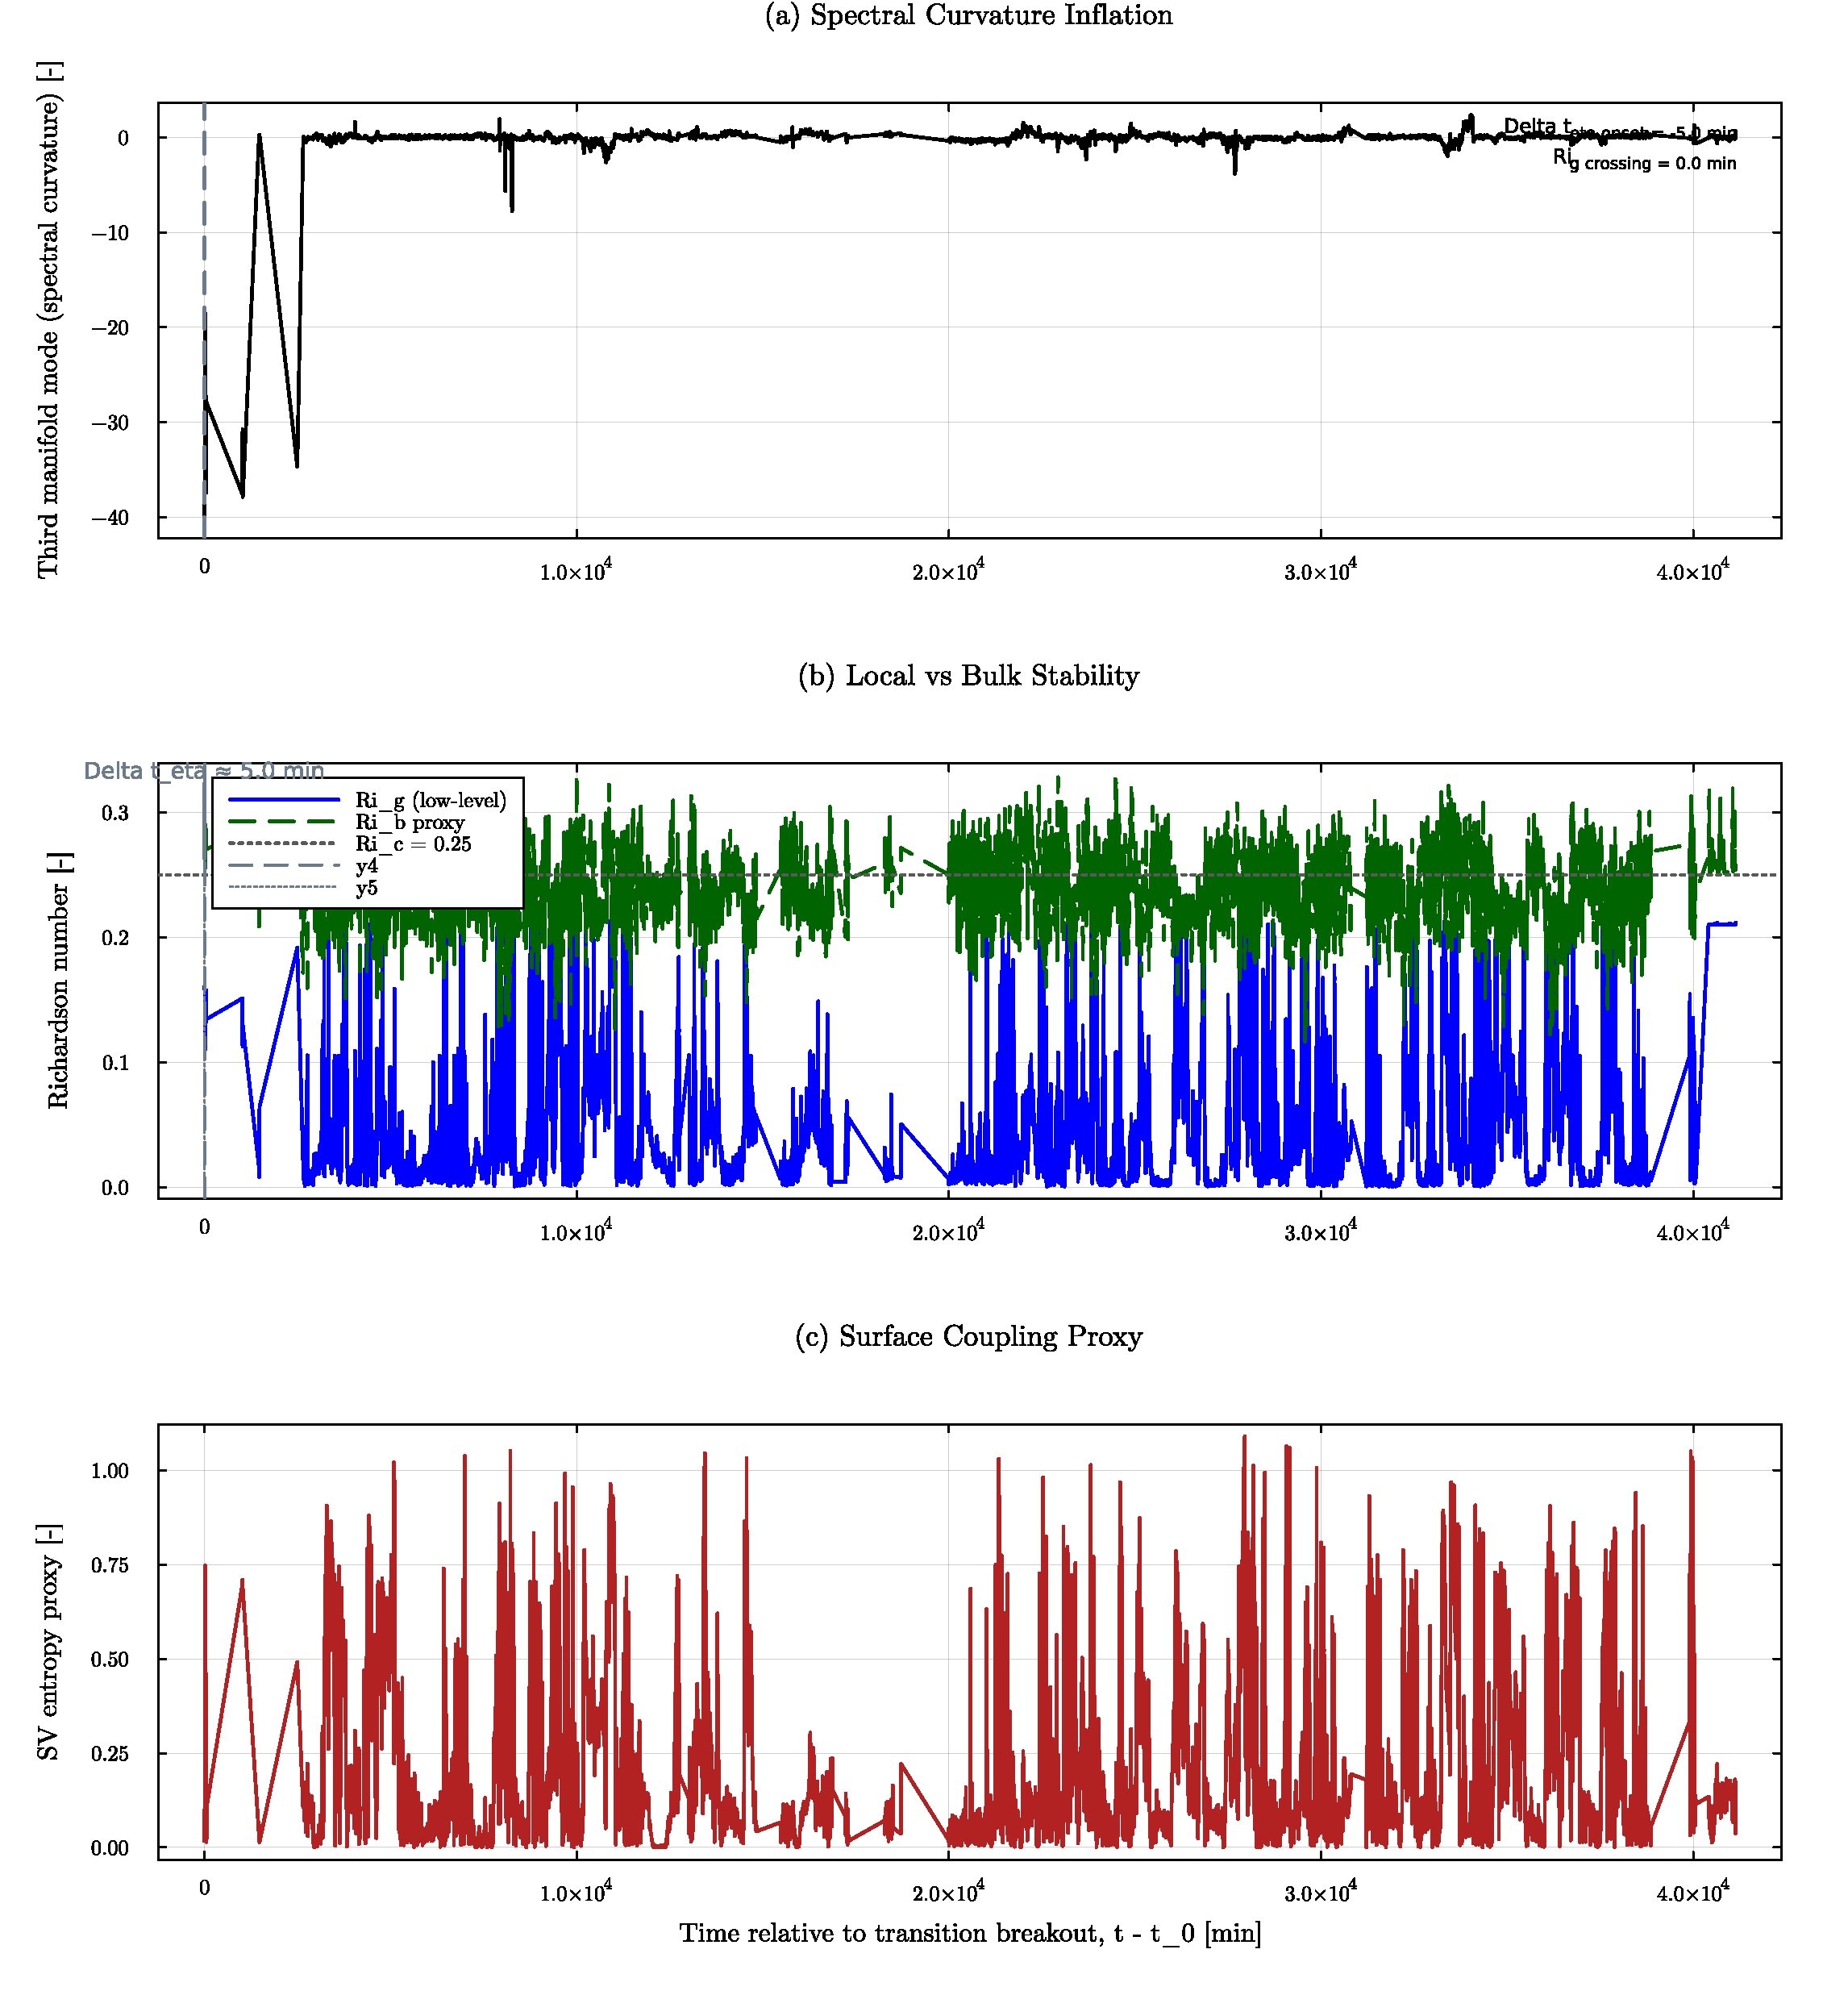
\includegraphics[width=\textwidth,height=0.82\textheight,keepaspectratio]{fig6_shadow_timeseries.pdf}
\caption{Structural-shadow timeseries (CASES-99). Smoothed curvature-onset diagnostics and lead-time brackets quantify precursor advance relative to local Richardson crossing.}
\label{fig:fig6-shadow}
\end{figure}

\begin{figure}[p]
\centering
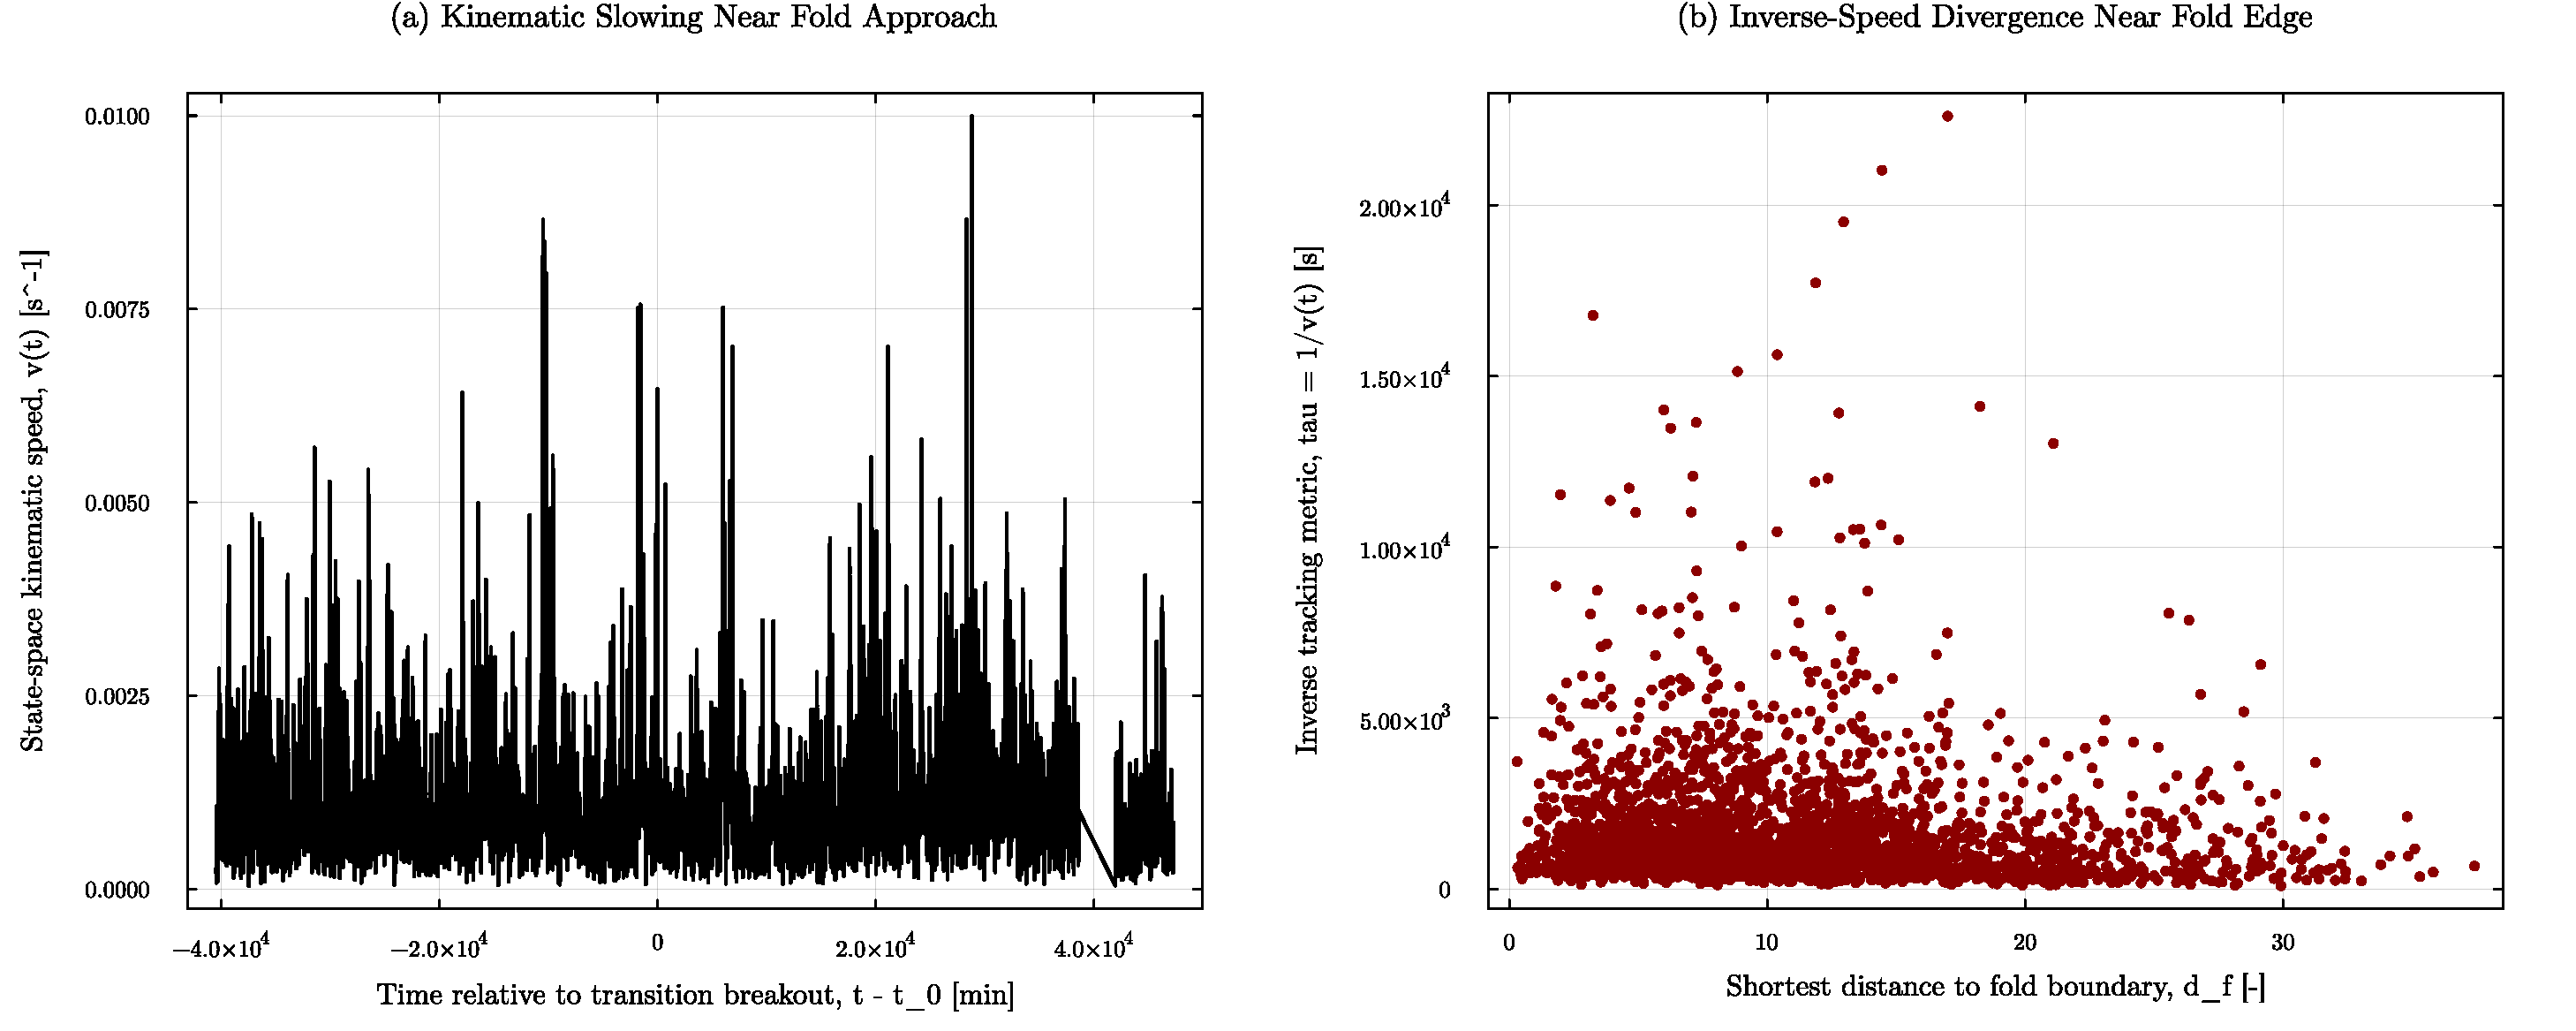
\includegraphics[width=\textwidth,height=0.82\textheight,keepaspectratio]{fig7_slowing_down.pdf}
\caption{Kinematic evidence of critical slowing near fold approach using orbital speed $s(t)$ and inverse-time metric $\tau=1/s$.}
\label{fig:fig7-slowing}
\end{figure}

\begin{figure}[p]
\centering
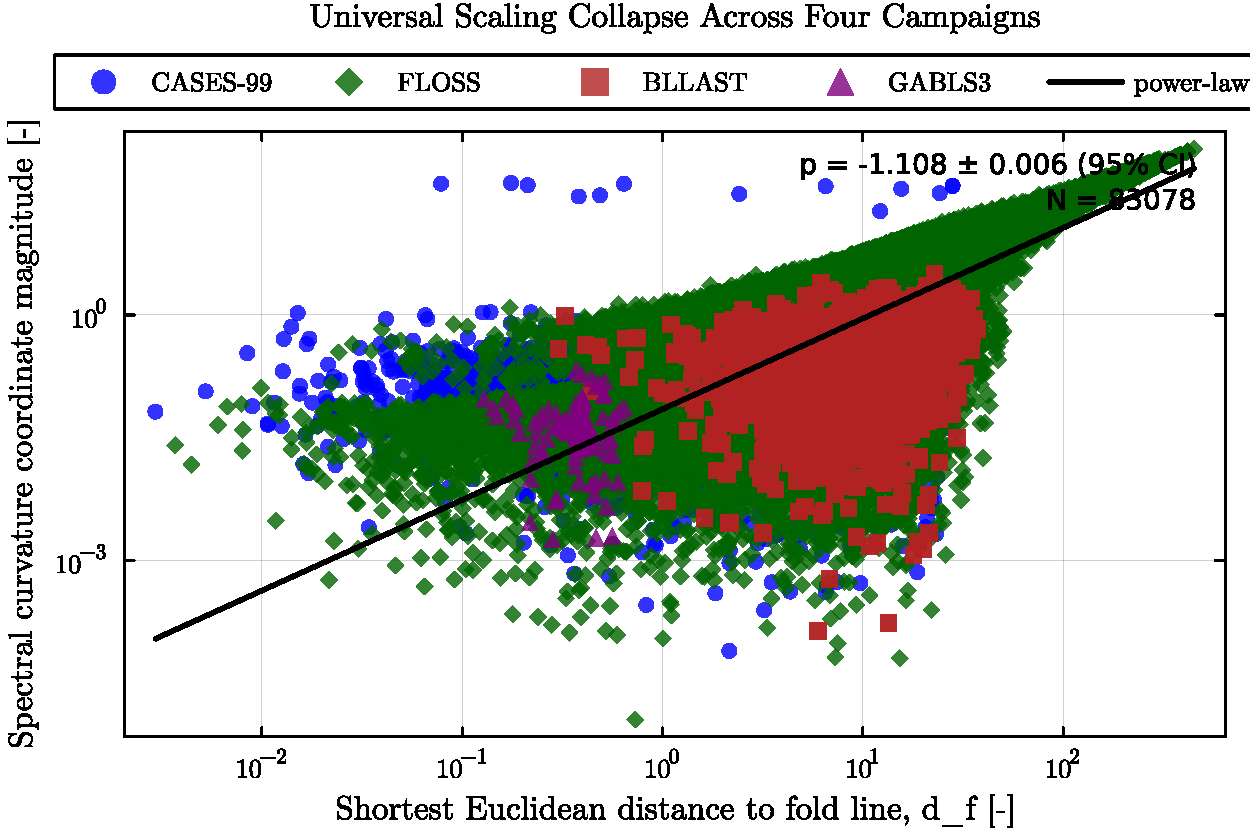
\includegraphics[width=\textwidth,height=0.82\textheight,keepaspectratio]{fig8_universal_collapse.pdf}
\caption{Universal collapse across campaigns with a power-law fit between fold-line distance and spectral curvature mode.}
\label{fig:fig8-collapse}
\end{figure}

\end{document}
